\section{Structure and Properties of Matter}

\begin{multicols}{2}

\section*{States of Matter} \label{sec:states-matter} \index{Matter! states of}
%All matter is made up of particles. These particles are in constant motion which increases with their temperature. Depending on temperature, matter may exist in three states: \emph{solid}, \emph{liquid} or \emph{gas}.


\subsection{Student Particles}

\begin{center}
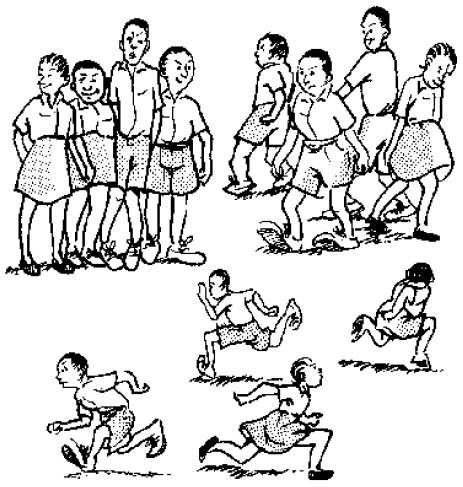
\includegraphics[width=0.4\textwidth]{./img/source/states-matter.png}
%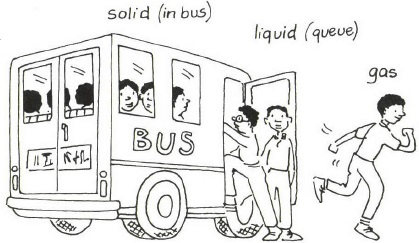
\includegraphics[width=0.4\textwidth]{./img/vso/states-matter.png}
\end{center}

\begin{description*}
%\item[Subtopic:]{}
%\item[Materials:]{}
%\item[Setup:]{}
\item[Procedure:]{Use students to demonstrate the concept of states of matter.}
%\item[Hazards:]{}
%\item[Questions:]{}
%\item[Observations:]{}
\item[Theory:]{When students or objects are close together, they represent particles in the \emph{solid} state. As they move apart and past each other they represent particles in the \emph{liquid} state. Fast and randomly moving pupils or objects represent particles in the \emph{gaseous} state.}
%\item[Applications:]{}
%\item[Notes:]{}
\end{description*}

\subsection{A Model of Motion}

\begin{center}
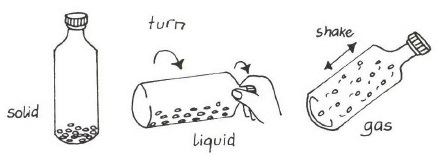
\includegraphics[width=0.49\textwidth]{./img/vso/motion-model.jpg}
\end{center}

\begin{description*}
%\item[Subtopic:]{}
%\item[Materials:]{}
%\item[Setup:]{}
\item[Procedure:]{Put some dry beans, rice or stones in a clear bottle. Hold the bottle still, then turn it, then shake it vigorously.}
%\item[Hazards:]{}
\item[Questions:]{Which activity corresponds to which state of matter?}
%\item[Observations:]{}
\item[Theory:]{The movement of particles in solids is small and hence they are in fixed order. In liquids the particles move past each other and have lost the stiff order. In gases they move very fast and randomly, losing all order.}
%\item[Applications:]{}
%\item[Notes:]{}
\end{description*}

\subsection{Changes of State} \index{Matter! states of}

\begin{center}
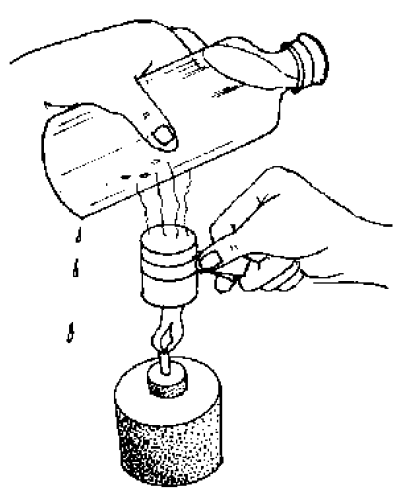
\includegraphics[width=0.25\textwidth]{./img/source/change-state.png}
\end{center}

\begin{description*}
%\item[Subtopic:]{}
\item[Materials:]{Tin can, glass bottle, water, \nameref{sec:heatsources}}
%\item[Setup:]{}
\item[Procedure:]{Pour a small amount of water into a tin can and heat it until it boils. Fill a bottle with cool water and hold it above the tin can.}
%\item[Hazards:]{}
%\item[Questions:]{}
\item[Observations:]{Water drops form on the outside of the cool bottle when it is touched by the steam of the boiling water.}
\item[Theory:]{Water particles escape from the boiling water as vapour and condense on the lower surface of the bottle to form water droplets. Hence water is made up of small particles.}
%\item[Applications:]{}
%\item[Notes:]{}
\end{description*}

\subsection{Model of Brownian Movement}

\begin{center}
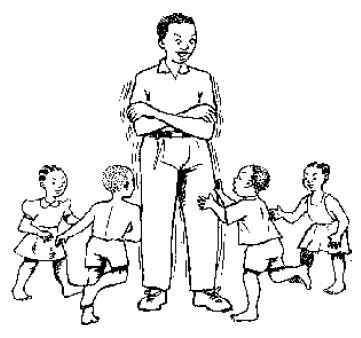
\includegraphics[width=0.4\textwidth]{./img/source/brownian.jpg}
\end{center}

Imagine there would be standing a tall adult person around whom small children are in a
continuous random movement. The tall person would be punched permanently by the
children and hence would be jerkily moved.

%\begin{description*}
%%\item[Subtopic:]{}
%\item[Materials:]{}
%\item[Setup:]{}
%\item[Procedure:]{}
%\item[Hazards:]{}
%\item[Questions:]{}
%\item[Observations:]{}
%\item[Theory:]{}
%\item[Applications:]{}
%\item[Notes:]{}
%\end{description*}

%\vfill
\columnbreak

%==================================================================================================%

\section*{Particulate Nature of Matter}


\subsection{Salt is Made of Particles}

\begin{center}
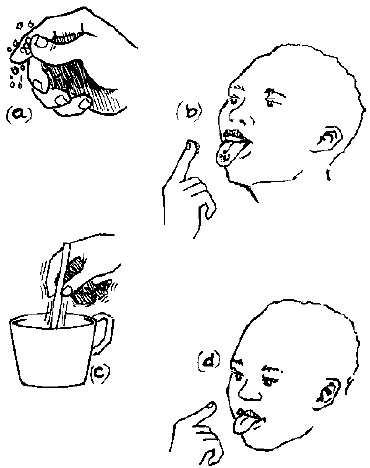
\includegraphics[width=0.4\textwidth]{./img/source/salt-particles.png}
\end{center}

\begin{description*}
%\item[Subtopic:]{}
\item[Materials:]{Salt/sugar, cup, water}
%\item[Setup:]{}
\item[Procedure:]{Roll some salt or sugar crystals between your fingers. Taste the crystals. Take a sip of the water. Now put the salt or sugar in the water and shake it. Taste again.}
%\item[Hazards:]{}
%\item[Questions:]{}
%\item[Observations:]{The crystals are hard and of cubical shape. They dissolve in water and the solution tastes like salt or sugar.}
\item[Theory:]{Sugar and salt are made up of tiny particles that can be identified by tasting even though they can not be seen in a solution.}
%\item[Applications:]{}
%\item[Notes:]{}
\end{description*}

\subsection{Weighing Particles}

\begin{center}
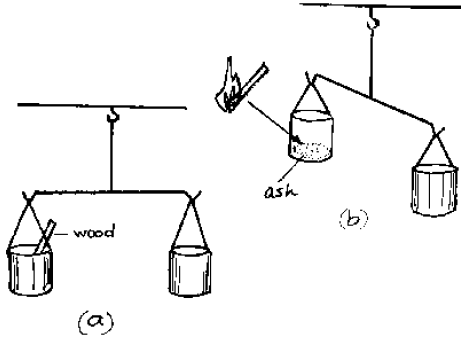
\includegraphics[width=0.49\textwidth]{./img/source/weighing-particles.png}
\end{center}

\begin{description*}
%\item[Subtopic:]{}
\item[Materials:]{\nameref{sec:balance}, small pieces of wood, \nameref{sec:heatsources}}
%\item[Setup:]{}
\item[Procedure:]{Weight pieces of wood and record the weight. Then burn the wood and weigh the ash.}
%\item[Hazards:]{}
\item[Questions:]{Is there a difference between the two weights?}
%\item[Observations:]{}
\item[Theory:]{The weight of the ash is less than that of wood. The loss in weight is due to particles which escaped as soot and gas.}
\item[Applications:]{This is why garbage reduces in size when burned. Burning wood and garbage releases carbon dioxide and other harmful gases into our environment. This is one form of \emph{pollution}.}
%\item[Notes:]{}
\end{description*}

%==================================================================================================%

\section*{Elasticity} \index{Elasticity}


\subsection{Hooke's Law} \index{Hooke's law|see{Practicals}} \index{Practicals! Hooke's law}
\textbf{*NECTA PRACTICAL*}
\begin{center}
%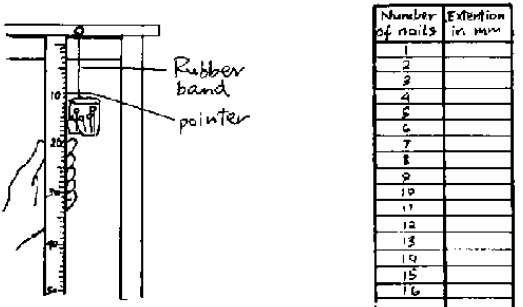
\includegraphics[width=0.49\textwidth]{./img/source/elasticity.png}
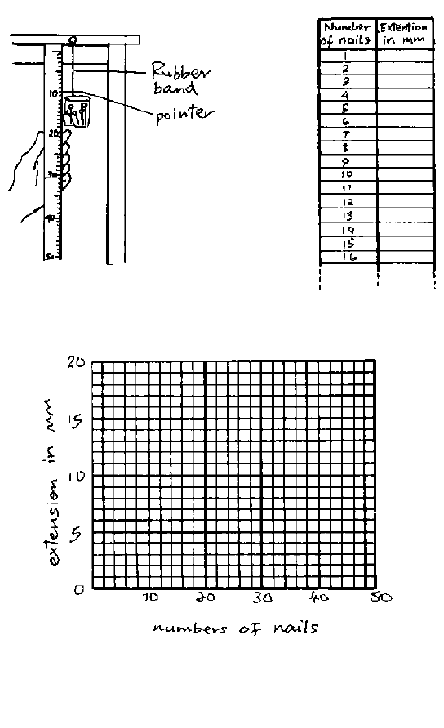
\includegraphics[width=0.49\textwidth]{./img/source/meas-mass.png}
\end{center}

\begin{description*}
%\item[Subtopic:]{}
\item[Materials:]{Rubber band/elastic strip, ruler, wire, \nameref{sec:scale-pan}, nails/small \nameref{sec:masses}, tape}
\item[Setup:]{Fix a ruler and rubber band side-by-side to a table or retort stand. At the other end of the rubber band, attach a small length of wire to act as a pointer and a small bag or scale pan (e.g. cardboard tube).}
\item[Procedure:]{Fill the scale pan with regular increments of nails or known weights. Have students measure the extension of the rubber band after each addition. Record and use the data to draw a graph of force (weight) against extension.}
%\item[Hazards:]{}
\item[Questions:]{What is the relationship between number of weights added and extension of the rubber band? What does the slope of the graph represent?}
%\item[Observations:]{}
\item[Theory:]{Hooke's Law states that the force applied to an elastic object is directly proportional to its extension ($F = kx$). The slope represents the elastic constant of the material. }
%\item[Applications:]{}
%\item[Notes:]{}
\end{description*}

%\vfill
\columnbreak

%==================================================================================================%

\section*{Adhesion and Cohesion} \index{Adhesion} \index{Cohesion}
Forces between particles of the same material are called \emph{cohesive forces} while those between particles of different materials are called \emph{adhesive forces}.


\subsection{Adhesion of Glass and Water}

\begin{center}
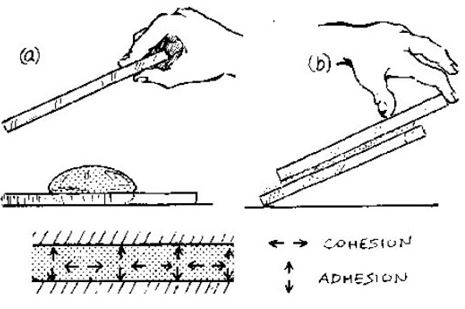
\includegraphics[width=0.49\textwidth]{./img/source/adhesion-cohesion.jpg}
\end{center}

\begin{description*}
%\item[Subtopic:]{}
\item[Materials:]{2 glass sheets, water, straw}
%\item[Setup:]{}
\item[Procedure:]{Drip water on a clean glass sheet (a). Place a second glass sheet on the wet first sheet and try to lift it (b).}
%\item[Hazards:]{}
%\item[Questions:]{}
%\item[Observations:]{}
\item[Theory:]{(a) Water spreads to form a patch on the first glass surface because \emph{adhesive forces}
attract water molecules to the glass surface.
(b) A strong force is required to separate the two glass sheets because the adhesive forces
between glass and water are large.}
%\item[Applications:]{}
%\item[Notes:]{}
\end{description*}

\subsection{Pinching Water}
\begin{description*}
%\item[Subtopic:]{}
\item[Materials:]{500 mL water bottle, needle/pin}
\item[Setup:]{Make 5 small holes at the bottom of the bottle with a syringe needle or nail. Make them close together (about 5 mm apart).}
\item[Procedure:]{Fill the bottle with water and allow it to flow through the holes at the bottom. Use your thumb and forefinger to pinch the streams together to form a single stream. Pass your hand over the holes and all five will appear again.}
%\item[Hazards:]{}
%\item[Questions:]{}
%\item[Observations:]{}
\item[Theory:]{Water has a tendency to cling to itself due to its surface tension and cohesion. As you bring the streams together, you allow the water to stick to itself forming a single stream. Passing your hand in front again stops the flow of water and allows it to start again in five streams.}
%\item[Applications:]{}
%\item[Notes:]{}
\end{description*}

\columnbreak

\subsection[Exploring Adhesion and Cohesion]{Exploring Adhesion and \hfill \\ Cohesion}

\begin{center}
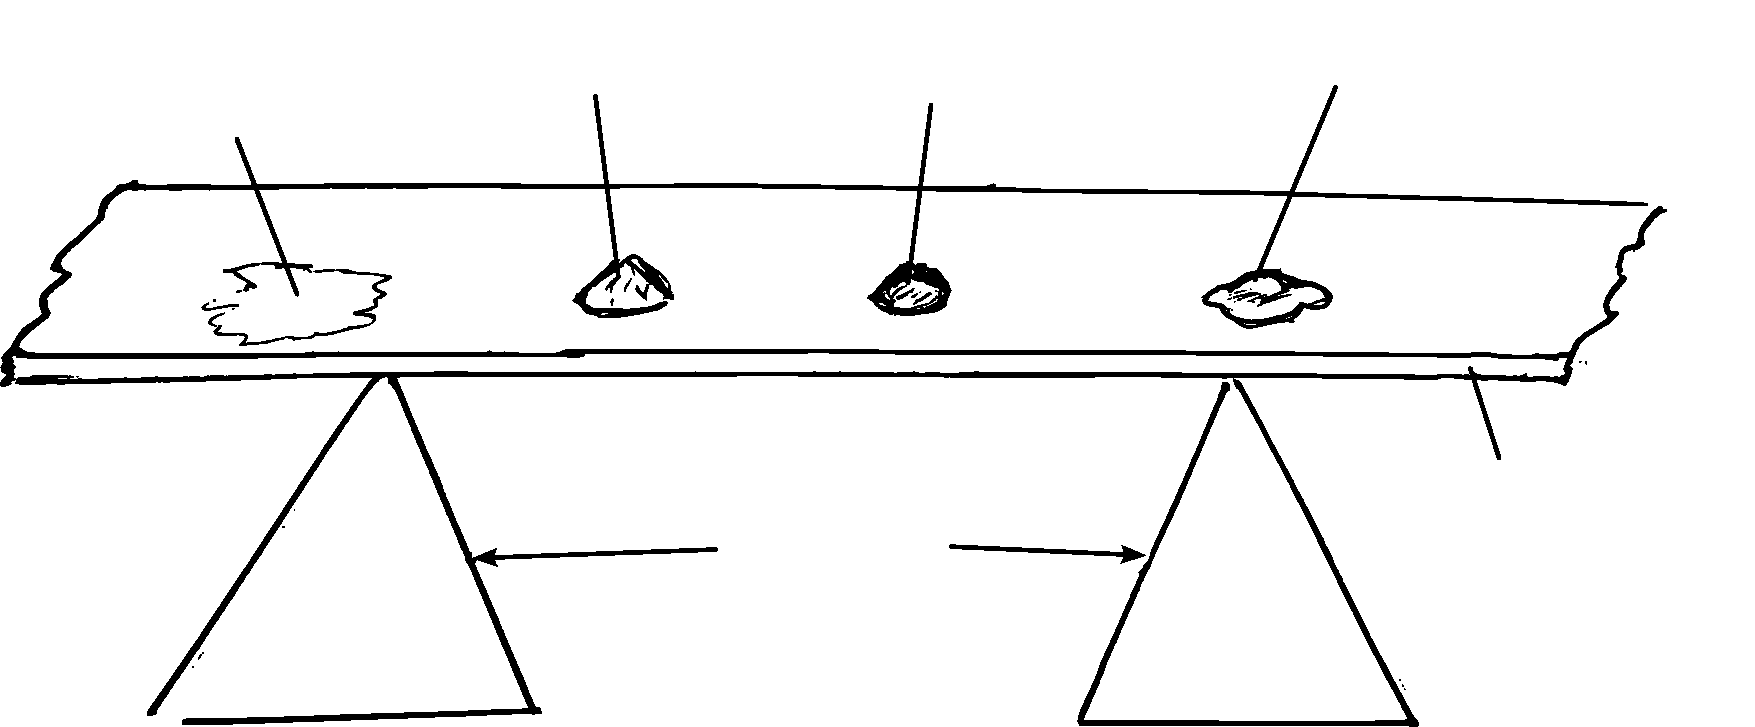
\includegraphics[width=0.45\textwidth]{./img/adhesion-cohesion.png}
\end{center}

\begin{description*}
%\item[Subtopic:]{}
\item[Materials:]{Sheet of glass, water, honey, glycerin, cooking oil, syringe, and 2 wooden blocks}
%\item[Setup:]{}
\item[Procedure:]{Place a sheet of glass over two wooden blocks on a table. Using a syringe, place a drop of different liquids on the glass.}
%\item[Hazards:]{}
%\item[Questions:]{}
\item[Observations:]{Water spreads and wets the glass, while honey, glycerin and cooking oil remain in a spherical shape.}
\item[Theory:]{The adhesive forces between the water molecules and glass molecules are greater, while the cohesive forces between the molecules of honey, glycerin and cooking oil are larger.}
%\item[Applications:]{}
%\item[Notes:]{}
\end{description*}

\subsection{Water Drops}

\begin{center}
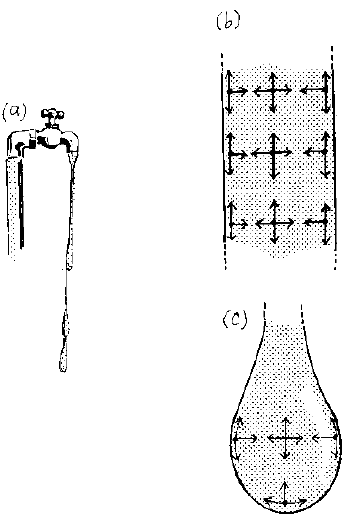
\includegraphics[width=0.3\textwidth]{./img/source/water-drops.png}
\end{center}

\begin{description*}
%\item[Subtopic:]{}
\item[Materials:]{Syringe or water dropper}
%\item[Setup:]{}
\item[Procedure:]{Slowly drip water from the syringe or water dropper. Observe how the drop forms.}
%\item[Hazards:]{}
%\item[Questions:]{}
\item[Observations:]{The water stream grows thinner and thinner as it moves further down and finally breaks to form drops.}
\item[Theory:]{Strong cohesive forces hold the water molecules together, until they are overcome by gravity and the water breaks off as drops.}
%\item[Applications:]{}
%\item[Notes:]{}
\end{description*}


\columnbreak

%==================================================================================================%

\section*{Surface Tension} \index{Surface tension}


\subsection{Water Dome}

\begin{center}
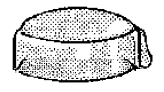
\includegraphics[width=0.2\textwidth]{./img/source/water-dome.png}
\end{center}

\begin{description*}
%\item[Subtopic:]{}
\item[Materials:]{Coin, water, syringe or eyedropper}
%\item[Setup:]{}
\item[Procedure:]{Place the coin flat on a table. Use the syringe or eyedropper to carefully drop individual water drops onto the coin.}
%\item[Hazards:]{}
\item[Questions:]{How many drops do you think the coin can hold?}
\item[Observations:]{The coin holds a surprising number of drops and forms a dome shape before the water spills over.}
\item[Theory:]{The surface tension of the water holds it together against the force of gravity, which is trying to pull the water off the coin.}
%\item[Applications:]{}
%\item[Notes:]{}
\end{description*}

\subsection{Pin Float}

\begin{center}
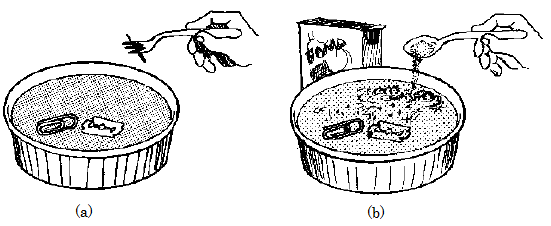
\includegraphics[width=0.49\textwidth]{./img/source/pin-float.png}
\end{center}

\begin{description*}
%\item[Subtopic:]{}
\item[Materials:]{Cup or small dish, straight pin/razor/paper clip, water, detergent}
%\item[Setup:]{}
\item[Procedure:]{Fill the cup with clean water and carefully float a pin, razor or small paper clip. Now add a small amount of detergent to the water and observe what happens.}
%\item[Hazards:]{}
%\item[Questions:]{}
\item[Observations:]{The objects float on the surface of the water initially, but after adding detergent, they sink to the bottom.}
\item[Theory:]{The surface tension of the water acts as an elastic membrane and is strong enough to support the small objects. Soap lowers the surface tension of water and therefore the objects sink.}
%\item[Applications:]{}
%\item[Notes:]{}
\end{description*}

\columnbreak

\subsection{Overflowing Glass}

\begin{center}
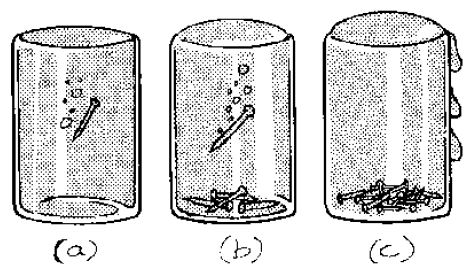
\includegraphics[width=0.45\textwidth]{./img/source/glass-overflow.jpg}
\end{center}

\begin{description*}
%\item[Subtopic:]{}
\item[Materials:]{Glass cup, water, nails}
%\item[Setup:]{}
\item[Procedure:]{Carefully fill a transparent glass vessel with water to the rim. Add nails, one at a time, to
the water and count the number of nails sunk just as water begins to spill over.}
%\item[Hazards:]{}
%\item[Questions:]{}
\item[Observations:]{The water surface bulges out but does not break immediately because of strong \emph{cohesion
forces} between the water particles.}
%\item[Theory:]{}
%\item[Applications:]{}
%\item[Notes:]{}
\end{description*}

\subsection{Blowing Bubbles}
\begin{description*}
%\item[Subtopic:]{}
\item[Materials:]{Thin piece of wire (approximately 30cm), water, detergent, glycerin (optional)}
\item[Setup:]{Bend the wire to form a loop of 2 to 3 cm in diameter, circling this loop many times. Leave a straight piece several cm long as a handle. Make a concentrated solution of detergent in water with a small amount of glycerin.}
\item[Procedure:]{Dip the circular part of the wire into the detergent. You should see a thin soapy film across the circle upon removal. Gently blow through the circle until a bubble separates from the wire.}
%\item[Hazards:]{}
%\item[Questions:]{}
\item[Observations:]{While blowing, the solution is being pulled back towards the surface. Once it breaks free as a bubble, it forms a spherical shape.}
\item[Theory:]{The surface tension of water causes the bubble to form the shape with the minimum surface area, which is a sphere.}
%\item[Applications:]{}
%\item[Notes:]{}
\end{description*}

\columnbreak

%==================================================================================================%

\section*{Capillarity} \index{Capillarity}


\subsection{Capillary Rise}

\begin{center}
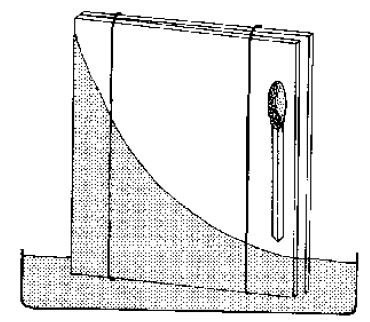
\includegraphics[width=0.4\textwidth]{./img/source/capillary-glass.jpg}
\end{center}

\begin{description*}
%\item[Subtopic:]{}
\item[Materials:]{2 glass sheets, match, rubber bands, water, food colour (optional)}
%\item[Setup:]{}
\item[Procedure:]{With the help of a rubber band and a matchstick, arrange two clean glass sheets as shown
in the diagram. Place the arrangement in a plate containing some water.}
%\item[Hazards:]{}
%\item[Questions:]{}
\item[Observations:]{Water rises to different heights along and between the glass sheets. }
\item[Theory:]{This is capillary
action. Capillary rise results from adhesion, allowing the liquid to climb along the surface of the glass, as well as cohesion, which pulls the remainder of the liquid up. Water rises more where the glass sheets are closer together.}
%\item[Applications:]{}
%\item[Notes:]{}
\end{description*}

%\subsection{Capillary Rise}
%
%\begin{center}
%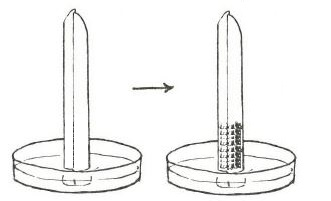
\includegraphics[width=0.4\textwidth]{./img/source/capillary-rise.jpg}
%\end{center}
%
%\begin{description*}
%%\item[Subtopic:]{}
%\item[Materials:]{Straws/chalk of different sizes, bottle, food colour, various liquids, e.g. water, spirit, kerosene, cooking oil}
%\item[Setup:]{Cut the bottom of a bottle to make a small dish.}
%\item[Procedure:]{Place one end of a straw/chalk into a dish of water 1 cm deep. Mark the change in level of the food colour after about a minute. Repeat for different liquids and different size straws.}
%%\item[Hazards:]{}
%\item[Questions:]{Which liquid rises the farthest up the straw? Do liquids rise faster in wide or thin straws?}
%\item[Observations:]{The spirit rises to the greatest height while water rises the least. Liquids rise faster in thin straws compared to thick ones.}
%\item[Theory:]{%Capillary rise results from adhesion, allowing the liquid to climb along the surface of the tube, as well as cohesion, which pulls the remainder of the liquid up. 
%In a thin container, a larger proportion of liquid is attached to the side of the tube and a smaller proportion is being held by surface tension, so the adhesive force is strong enough to pull more liquid up the tube.}
%%\item[Applications:]{}
%%\item[Notes:]{}
%\end{description*}

\subsection{Moving Matches}

%\begin{center}
%\includegraphics[width=0.4\textwidth]{./img/.png}
%\end{center}

\begin{description*}
%\item[Subtopic:]{}
\item[Materials:]{Matches, water, straw, plastic lid}
%\item[Setup:]{}
\item[Procedure:]{Break several matches near the middle, but not so that they come apart. They should make acute angles. Place them on the plastic lid and place a few drops of water on the broken joints of the matches using the straw.}
%\item[Hazards:]{}
%\item[Questions:]{}
\item[Observations:]{The matches close and return to their original straight shape.}
\item[Theory:]{Water gets absorbed in the wooden matchstick and causes it to expand.}
\item[Applications:]{This is why it is difficult to open a wooden door after it rains. The water rises up the wood causing it to expand into its frame.}
%\item[Notes:]{}
\end{description*}

\columnbreak

\subsection{Measuring Capillary Rise}

\begin{center}
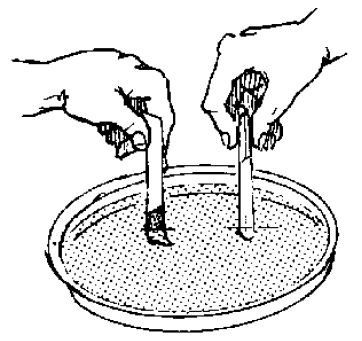
\includegraphics[width=0.4\textwidth]{./img/source/capillary-rise-meas.jpg}
\end{center}

\begin{description*}
%\item[Subtopic:]{}
\item[Materials:]{Paper, chalk, small dish/lid, water, food colour}
\item[Setup:]{Cut off the bottom of a plastic bottle to make a water dish.}
\item[Procedure:]{Place a strip of paper and a piece of chalk in a dish containing water. Leave the objects for some time and measure the rise in colour of each using a ruler.}
%\item[Hazards:]{}
%\item[Questions:]{}
\item[Observations:]{The water rises faster in the chalk than in the paper.}
\item[Theory:]{Chalk has smaller capillaries than paper, which allows water to rise faster.}
%\item[Applications:]{}
%\item[Notes:]{}
\end{description*}

\subsection{Automatic Irrigation}

\begin{center}
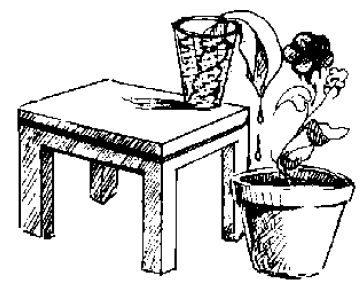
\includegraphics[width=0.3\textwidth]{./img/source/irrigation.png}
\end{center}

\begin{description*}
%\item[Subtopic:]{}
%\item[Materials:]{}
%\item[Setup:]{}
%\item[Procedure:]{}
%\item[Hazards:]{}
%\item[Questions:]{}
%\item[Observations:]{}
%\item[Theory:]{}
\item[Applications:]{Capillary action can be used to provide automatic irrigation for plants. Students can perform irrigation by dipping a porous material such as paper or cotton cloth in water.}
%\item[Notes:]{}
\end{description*}

\columnbreak

%==================================================================================================%

\section*{Diffusion} \index{Diffusion}

\subsection{Diffusion in Liquids}

\begin{center}
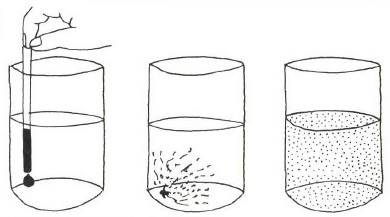
\includegraphics[width=0.4\textwidth]{./img/vso/diffusion.jpg}
\end{center}

\begin{description*}
%\item[Subtopic:]{}
\item[Materials:]{Plastic water bottle, food colour (liquid or powder)}
%\item[Setup:]{}
\item[Procedure:]{Put a drop or small amount of powdered food colour into the water without shaking and observe what happens.}
%\item[Hazards:]{}
%\item[Questions:]{}
\item[Observations:]{The colour gradually spreads throughout the water.}
\item[Theory:]{This spreading is due to the motion of the particles of food colour. This process is called \emph{diffusion}.}
\item[Applications:]{Organisms utilize diffusion to balance nutrient concentrations in cells and to transfer oxygen into the bloodstream during respiration.}
%\item[Notes:]{}
\end{description*}

\subsection{Smelling Particles}

\begin{center}
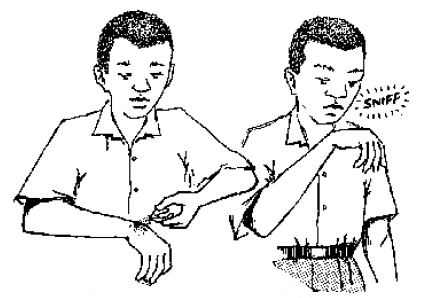
\includegraphics[width=0.4\textwidth]{./img/source/smelling-particles.jpg}
\end{center}

\begin{description*}
%\item[Subtopic:]{}
\item[Materials:]{Orange or other citrus fruit, box}
%\item[Setup:]{}
\item[Procedure:]{Peel and orange and have students raise their hands when they begin to smell it. Now place a box in front of the orange and repeat the test.}
%\item[Hazards:]{}
%\item[Questions:]{}
\item[Observations:]{Students in the front center of the room should be the first to raise their hands, followed by those near the sides and in the back. When the orange is peeled behind the box it takes longer for the smell to reach the students.}
\item[Theory:]{Tiny particles from the orange peel spread by diffusion to students' noses. The box hinders the motion of the particles and so they reach the students more slowly.}
\item[Applications:]{Air fresheners and other sprays}
%\item[Notes:]{}
\end{description*}

\subsection{Diffusion in Daily Life}

\begin{center}
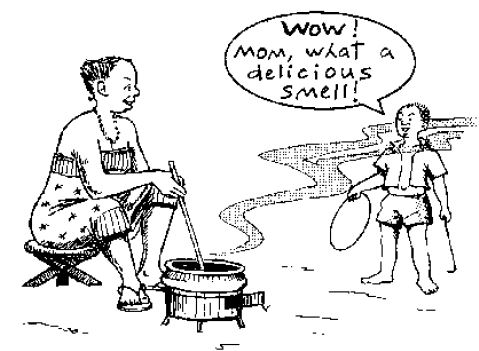
\includegraphics[width=0.49\textwidth]{./img/source/diffusion-life.jpg}
\end{center}

\begin{description*}
%\item[Subtopic:]{}
%\item[Materials:]{}
%\item[Setup:]{}
\item[Procedure:]{Pass near a place where people are roasting meat or cooking.}
%\item[Hazards:]{}
%\item[Questions:]{}
%\item[Observations:]{}
\item[Theory:]{The smell is sensed even at a distance, because the particles which produce the smell
spread by \emph{diffusion}.}
%\item[Applications:]{}
%\item[Notes:]{}
\end{description*}

\subsection{Diffusion and Pollution} \index{Pollution}

\begin{center}
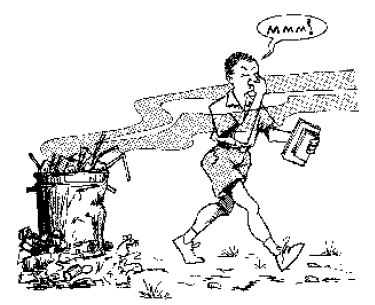
\includegraphics[width=0.49\textwidth]{./img/source/diffusion-pollution.jpg}
\end{center}

\begin{description*}
%\item[Subtopic:]{}
%\item[Materials:]{}
%\item[Setup:]{}
\item[Procedure:]{Pass near a polluted area (e.g. latrine, burning heaps of litter, a filling station).}
%\item[Hazards:]{}
%\item[Questions:]{}
%\item[Observations:]{}
\item[Theory:]{Many hazardous substances spread to the environment by diffusion. (Hazardous
substances in any state of matter in our environment mean pollution.)}
%\item[Applications:]{}
%\item[Notes:]{}
\end{description*}

\columnbreak

%==================================================================================================%

\section*{Osmosis} \index{Osmosis}


\subsection{Vanilla Balloon}

\begin{center}
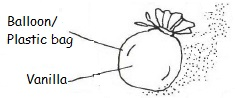
\includegraphics[width=0.35\textwidth]{./img/vso/osmosis-vanilla.jpg}
\end{center}

\begin{description*}
%\item[Subtopic:]{}
\item[Materials:]{Balloon/plastic bag, vanilla, straw/syringe}
%\item[Setup:]{}
\item[Procedure:]{Place a few drops of vanilla in a deflated balloon. Now blow up the balloon and tie it shut.}
%\item[Hazards:]{}
%\item[Questions:]{}
\item[Observations:]{You can smell the vanilla through the surface of the balloon.}
\item[Theory:]{The balloon acts as a \emph{semi-permeable membrane} which allows some of the vanilla particles to pass through and reach your nose. Other particles remain inside the balloon.}
%\item[Applications:]{}
%\item[Notes:]{}
\end{description*}

\subsection{Potato Osmosis}

\begin{center}
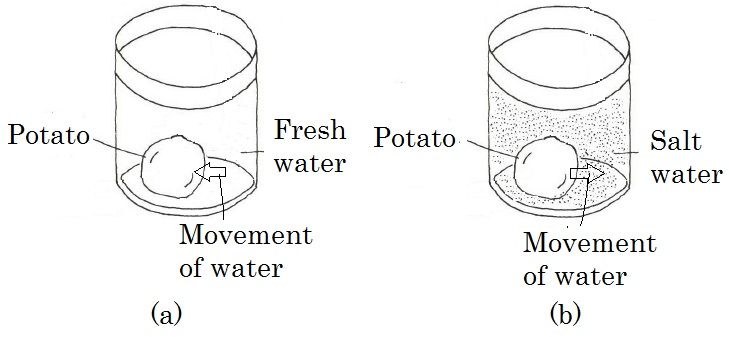
\includegraphics[width=0.49\textwidth]{./img/vso/osmosis-potato-full.jpg}
\end{center}

\begin{description*}
%\item[Subtopic:]{}
\item[Materials:]{Potato, 2 water bottles, salt, water}
\item[Setup:]{Cut two equal size pieces of potato. Fill one bottle with fresh water and the other with a salt water solution.}
\item[Procedure:]{Put one piece of potato in each bottle. Observe over the next few hours.}
%\item[Hazards:]{}
%\item[Questions:]{}
\item[Observations:]{The potato in fresh water swells while the potato in salt water shrivels up.}
\item[Theory:]{Through osmosis, water moves from a region of low concentration to one of high concentration through a semi-permeable membrane (the potato). In fresh water, the potato has the higher salt concentration, so water enters in order to make a balance. In salt water, the concentration of the surrounding water is higher than that of the potato, so water inside the potato moves outside to dilute the salt solution.}
%\item[Applications:]{}
\item[Notes:]{Try this experiment again with a boiled potato. Do you observe any differences?}
\end{description*}

\columnbreak

\subsection{Semi-Permeable Membranes}

\begin{center}
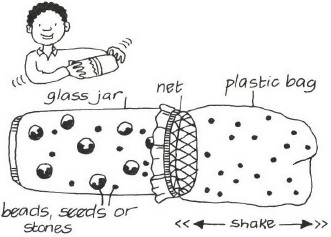
\includegraphics[width=0.4\textwidth]{./img/vso/membrane.jpg}
\end{center}

\begin{description*}
%\item[Subtopic:]{}
\item[Materials:]{Glass jar, clear plastic bag, small beads or stones, beans, netting, string/rubber band}
\item[Setup:]{Place the mixture of beads and beans in the jar. Place the net and plastic bag over the top and tie them on securely.}
\item[Procedure:]{Shake the apparatus for a few seconds.}
%\item[Hazards:]{}
%\item[Questions:]{}
\item[Observations:]{Only the small beads pass through the netting. The beans remain in the jar.}
\item[Theory:]{The beads represent small molecules and the net is a semi-permeable membrane. The beans are too large to pass through and hence remain in the jar.}
\item[Applications:]{Water filters, organism cell membranes}
%\item[Notes:]{}
\end{description*}

\subsection{Osmosis with Eggs} % VSO 25

\begin{center}
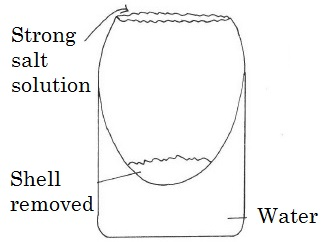
\includegraphics[width=0.4\textwidth]{./img/vso/osmosis-eggs.jpg}
\end{center}

\begin{description*}
%\item[Subtopic:]{}
\item[Materials:]{Empty eggshell, strong salt solution, jar of water}
%\item[Setup:]{}
\item[Procedure:]{Remove the hard outer shell at
one end of the eggshell to
expose the inner membrane. Half
fill the egg with salt solution and
place it in the jar so that the
water level is above the exposed
membrane and leave for a couple
of hours. }
%\item[Hazards:]{}
\item[Observations:]{The level of
the solution inside the egg rises,
indicating water has crossed the
membrane, i.e. osmosis has
occurred.}
%\item[Questions:]{What happens if you use sugar solution instead of salt? What if you put salt solution in the jar as well as the egg?}
\item[Theory:]{Water travels from an area of low concentration to an area of high concentration of salts.}
%\item[Applications:]{}
%\item[Notes:]{}
\end{description*}


\end{multicols}

\pagebreak